\section{Resultados}

El proceso de selección de datos arrojó 16661 ítems con sus respectivas bolsas de palabras, que luego pasaron por un procesamiento de texto 
en rapidminer para crear un vector de palabras de TF-IDF.\\
Dicho vector estaba quedó conformado por una matriz de 16661 filas, representando a cada ítem y 49098 columnas, una por cada palabra encontrada 
en almenos un ítem.\\
En base a ese vector, se ejecutaron todos los algoritmos de clustering de distintas configuraciones para el k-medias, utilizando valores de K de 9,10,11,13,17,20,25 y 30. 
También utilizando divergencia de Bregman y como medida de distancia la distancia euclideana cuadrada.\\
El tiempo de ejecución para dichos algoritmos aumentaba, a medida que aumentaba la cantidad de centroides configurados, partiendo desde 10 horas para 
el más corto y 36 horas para el más largo.\\
\\
Una vez concluidos exitosamente todos los algoritmos se procedió a ejecutar el algoritmo de cálculo de silhouette index.\\
Puede observarse en la imagen, que existe una tendencia a mejorar la performance del modelo a medida que el número de centroides 
(K) aumenta. Lo que implica que se debería seguir aumentando dicha configuración, según el índice.


Luego el proceso de análisis manual, dio un panorama mucho más revelador, que el índice.\\
Sobretodo porque se pudieron evaluar aspectos mucho más importantes en consideración a la finalidad de haber realizado el clustering.\\
En Figure 1: Performances por cantidad de centroides se disponen de los resultados de los análisis de cada modelo.\\
\\
Se debe tener en cuenta qué, Cluster es simplemente el número identificador del cluster, Población se refiere a la cantidad de ítems 
dentro del cluster, Tipo es el tipo que humanamente le fue otorgado al cluster (teniendo en considerando que fue necesario realizar una 
abstracción adecuada, por ejemplo muchos clusters que contenían Alfombras para auto, fueron etiquetados como accesorios para Auto), Efectivos 
es la cantidad de ítems dentro del cluster que pertenecían a ese tipo (Observar que un cluster puede contener ítems de múltiples tipos, pero el tipo 
etiquetado al claster representa a la mayoría), y utilidad significa si dicho tipo esta contenido en la ontología de schema.\\
\\
Modelo K9\\
\begin{tabular}{| c | c | c | c | c |}\hline
Cluster & Población & Tipo & Efectivos & Útiles\\\hline
0 & 2240 & Accesorios auto & 2240 & No\\
1 & 601 & Comida & 601 & No\\
2 & 2491 & Vestidos & 2491 & No\\
3 & 963 & Música & 963 & Sí\\
4 & 399 & Accesorios auto & 399 & No\\
5 & 512 & Cuchillos & 512 & No\\
6 & 1714 & Autos & 1714 & Sí\\
7 & 5031 & Libros & 1710 & Sí\\
8 & 2710 & Películas & 1978 & Sí\\\hline
\end{tabular}
\\
\\
Modelo K10\\
\begin{tabular}{| c | c | c | c | c |}\hline
Cluster & Población & Tipo & Efectivos & Útiles\\\hline
0 & 2491 & Vestidos & 2491 & No\\
1 & 536 & Accesorios auto & 536 & No\\
2 & 877 & Accesorios auto & 877 & No\\
3 & 513 & Cuchillos & 513 & No\\
4 & 601 & Comida & 601 & No\\
5 & 945 & Accesorios auto & 945 & No\\
6 & 6191 & Libros & 3590 & Sí\\
7 & 238 & Accesorios auto & 238 & No\\
8 & 2552 & Películas & 1709 & Sí\\
9 & 1717 & Autos & 1717 & Sí\\\hline
\end{tabular}
\\
\\
Modelo K12\\
\begin{tabular}{| c | c | c | c | c |}\hline
Cluster & Población & Tipo & Efectivos & Útiles\\\hline
0 & 609 & Accesorios auto & 609 & No\\
1 & 1423 & Accesorios auto & 1423 & No\\
2 & 1641 & Libros & 1641 & Sí\\
3 & 2702 & Películas & 2242 & Sí\\
4 & 3499 & Películas & 699 & Sí\\
5 & 1885 & Vestidos & 1885 & No\\
6 & 1699 & Autos & 1699 & Sí\\
7 & 601 & Comida & 601 & Sí\\
8 & 499 & Cuchillos & 499 & No\\
9 & 968 & Música & 968 & Sí\\
10 & 658 & Vestidos & 658 & No\\
11 & 477 & Accesorios auto & 477 & No\\\hline
\end{tabular}
\\
\\
Modelo K13\\
\begin{tabular}{| c | c | c | c | c |}\hline
Cluster & Población & Tipo & Efectivos & Útiles\\\hline
0 & 601 & Comida & 601 & No\\
1 & 1462 & Películas & 1462 & Sí\\
2 & 1717 & Autos & 1717 & Sí\\
3 & 513 & Cuchillos & 513 & No\\
4 & 2345 & Accesorios auto & 1336 & No\\
5 & 3801 & Libros & 1634 & Sí\\
6 & 357 & Accesorios auto & 357 & No\\
7 & 876 & Accesorios auto & 876 & No\\
8 & 2492 & Vestidos & 2492 & No\\
9 & 613 & Accesorios auto & 613 & No\\
10 & 238 & Accesorios auto & 238 & No\\
11 & 944 & Música & 944 & Sí\\
12 & 702 & Series & 702 & Sí\\\hline
\end{tabular}\\
\\
Modelo K17\\
\begin{tabular}{| c | c | c | c | c |}\hline
Cluster & Población & Tipo & Efectivos & Útiles\\\hline
0 & 1701 & Autos & 1701 & Sí\\
1 & 216 & Accesorios auto & 216 & No\\
2 & 896 & Música & 896 & Sí\\
3 & 434 & Cuchillos & 434 & No\\
4 & 585 & Accesorios auto & 585 & No\\
5 & 229 & Accesorios auto & 229 & No\\
6 & 240 & Hardware & 120 & Sí\\
7 & 239 & Accesorios auto & 239 & No\\
8 & 1216 & Películas & 1216 & Sí\\
9 & 1899 & Libros & 1709 & Sí\\
10 & 601 & Comida & 601 & No\\
11 & 887 & Accesorios auto & 887 & No\\
12 & 2465 & Vestidos & 2465 & No\\
13 & 184 & Cuchillos & 132 & No\\
14 & 600 & Accesorios auto & 600 & No\\
15 & 648 & Series & 648 & Sí\\
16 & 3621 & Películas & 832 & Sí\\\hline
\end{tabular}\\
\\
Modelo K20\\
\begin{tabular}{| c | c | c | c | c |}\hline
Cluster & Población & Tipo & Efectivos & Útiles\\\hline
0 & 465 & Accesorios auto & 246 & No\\
1 & 80 & Accesorios auto & 80 & No\\
2 & 3874 & Películas & 1045 & Sí\\
3 & 1629 & Libros & 1629 & Sí\\
4 & 2480 & Vestidos & 2480 & No\\
5 & 91 & Accesorios auto & 91 & No\\
6 & 238 & Accesorios auto & 238 & No\\
7 & 802 & Accesorios auto & 802 & No\\
8 & 601 & Comida & 601 & No\\
9 & 295 & Accesorios auto & 295 & No\\
10 & 396 & Accesorios auto & 396 & No\\
11 & 280 & Cuchillos & 280 & No\\
12 & 1282 & Películas & 1282 & Sí\\
13 & 311 & Videojeugos & 311 & Sí\\
14 & 47 & Autos & 47 & Sí\\
15 & 216 & Accesorios auto & 216 & No\\
16 & 675 & Accesorios auto & 675 & No\\
17 & 306 & Cuchillos & 306 & No\\
18 & 921 & Música & 921 & Sí\\
19 & 1672 & Autos & 1672 & Sí\\\hline
\end{tabular}\\
\\
Modelo K25\\
\begin{tabular}{| c | c | c | c | c |}\hline
Cluster & Población & Tipo & Efectivos & Útiles\\\hline
0 & 496 & Cuchillos & 496 & No\\
1 & 117 & Accesorios auto & 94 & No\\
2 & 884 & Música & 884 & Sí\\
3 & 167 & Accesorios auto & 167 & No\\
4 & 599 & Accesorios auto & 599 & No\\
5 & 352 & Series & 352 & Sí\\
6 & 225 & Accesorios auto & 225 & No\\
7 & 1710 & Autos & 1710 & Sí\\
8 & 2708 & Películas & 1354 & Sí\\
9 & 372 & Vestidos & 372 & No\\
10 & 1085 & Vestidos & 1085 & No\\
11 & 393 & Accesorios auto & 393 & No\\
12 & 655 & Accesorios auto & 655 & No\\
13 & 214 & Accesorios auto & 214 & No\\
14 & 480 & Series & 480 & Sí\\
15 & 80 & Accesorios auto & 80 & No\\
16 & 307 & Videojeugos & 307 & No\\
17 & 2213 & Libros & 1881 & Sí\\
18 & 135 & Accesorios auto & 108 & No\\
19 & 293 & Accesorios auto & 293 & No\\
20 & 1074 & Vestidos & 1074 & No\\
21 & 601 & Comida & 601 & No\\
22 & 1050 & Películas & 1050 & Sí\\
23 & 70 & Libros & 31 & Sí\\
24 & 381 & Accesorios auto & 381 & No\\\hline
\end{tabular}\\
\\
Modelo K30\\
\begin{tabular}{| c | c | c | c | c |}\hline
Cluster & Población & Tipo & Efectivos & Útiles\\\hline
0 & 443 & Música & 443 & Sí\\
1 & 1101 & Libros & 1101 & Sí\\
2 & 186 & Accesorios auto & 186 & No\\
3 & 295 & Accesorios auto & 295 & No\\
4 & 484 & Cuchillos & 484 & No\\
5 & 691 & Vestidos & 691 & No\\
6 & 91 & Accesorios auto & 91 & No\\
7 & 237 & Accesorios auto & 237 & No\\
8 & 1595 & Accesorios auto & 669 & No\\
9 & 857 & Vestidos & 857 & No\\
10 & 183 & Accesorios auto & 183 & No\\
11 & 601 & Comida & 601 & No\\
12 & 382 & Accesorios auto & 382 & No\\
13 & 860 & Películas & 860 & Sí\\
14 & 641 & Vestidos & 641 & No\\
15 & 590 & Libros & 590 & Sí\\
16 & 644 & Series & 644 & Sí\\
17 & 230 & Accesorios auto & 230 & No\\
18 & 80 & Accesorios auto & 80 & No\\
19 & 210 & Hardware & 138 & Sí\\
20 & 643 & Autos & 643 & Sí\\
21 & 477 & Accesorios auto & 477 & No\\
22 & 1740 & Películas & 1531 & Sí\\
23 & 1123 & Autos & 1123 & Sí\\
24 & 245 & Accesorios auto & 245 & No\\
25 & 352 & Vestidos & 352 & No\\
26 & 307 & Videojuegos & 282 & Sí\\
27 & 117 & Accesorios auto & 84 & No\\
28 & 774 & Hardware & 774 & Sí\\
29 & 482 & Música & 482 & Sí\\\hline
\end{tabular}
\\
\\
Evaluando entonces el conjunto de clusters de cada model, se puede obtener la siguiente tabla comparativa:\\
\begin{tabular}{| c | c | c | c | c |}\hline
Modelo & \%Etiquetas & \%etiquetas correctas & \%Efectividad & \%Redundancia\\ \hline
9 & 62 & 38 & 75 & 11\\
10 & 62 & 42 & 79 & 30\\
12 & 66 & 47 & 80 & 33\\
13 & 51 & 38 & 80 & 30\\
17 & 61 & 42 & 81 & 41\\
20 & 58 & 41 & 81 & 55\\
25 & 56 & 46 & 89 & 60\\
30 & 53 & 51 & 92 & 63\\ \hline
\end{tabular}

Donde, Modelo, es la cantidad de centroides del modelo, \%Etiquetas es el porcentaje de ítems etiquetados, \%etiquetas correctas es el porcentaje 
de ítems corréctamente etiquedatos, \%Efectividad es el porcentaje de ítems que fueron correctamente agrupados en los clusters. Y \%Redundancia 
es el porcentaje de clústers representando el mismo tipo.\\
\\
Se puede apreciar en Figure 2:Estadísticas por cantidad de centroides el gráfico estadístico obtenido en la última tabla.\\
Y también como disminuye el porcentaje de error en el etiquetado al aumentar la cantidad de centroides e nFigure 3: \% de etiquetas incorrectas por modelo
\begin{figure}
  \centering
    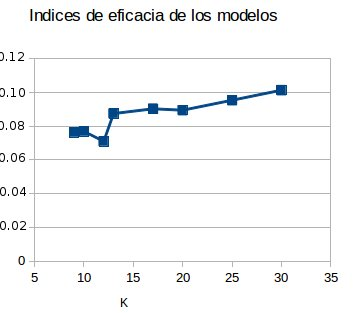
\includegraphics[width=0.7\textwidth]{chart1}
  \caption{Performances por cantidad de centroides}
  \label{fig:ejemplo}
\end{figure}
\begin{figure}
  \centering
    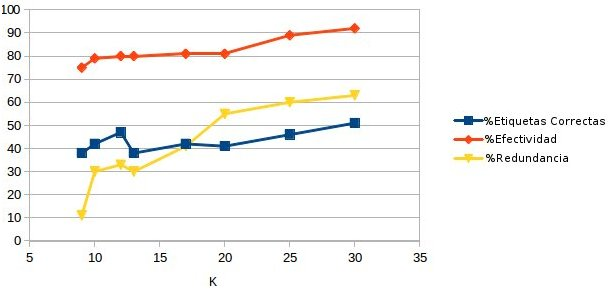
\includegraphics[width=0.7\textwidth]{chart2}
  \caption{Estadísticas por cantidad de centroides}
  \label{fig:ejemplo}
\end{figure}
\begin{figure}
  \centering
    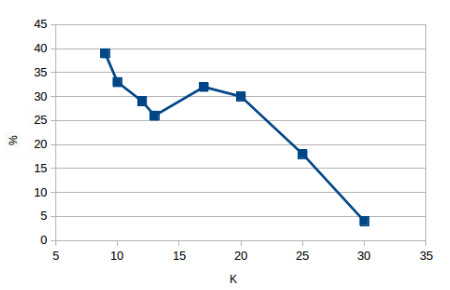
\includegraphics[width=0.7\textwidth]{char3}
  \caption{\% de etiquetas incorrectas por modelo}
  \label{fig:ejemplo}
\end{figure}
\\
\\
Dado que la necesidad de realizar un clustering está dada por la cantidad de ítems correctamente etiquetables bajo la ontología de schema, 
y no por nigún otro parámetro de evaluación, queda entonces decidido por una diferencia notoria el modelo resultanto por el algoritmo de k-medias 
con 30 centroides.
